\documentclass[12pt]{article}
\usepackage[letterpaper,margin=1in]{geometry}
\usepackage{times}
\usepackage{graphicx}
\usepackage{float}
\usepackage{booktabs}
\usepackage{amsmath,amssymb}
\usepackage[numbers,sort&compress]{natbib}
\usepackage[hyphens]{url}
\usepackage{setspace}
\usepackage[pagewise]{lineno}
\usepackage{array}
\usepackage{caption}

\doublespacing
\linenumbers
\urlstyle{same}

\newcommand{\D}{\mathcal{D}}
\newcommand{\Sset}{\mathcal{S}}
\newcommand{\Aset}{\mathcal{A}}
\newcommand{\Bset}{\mathcal{B}}
\newcommand{\Vset}{\mathcal{V}}

\title{Validation-Aligned Coreset Selection for Budgeted Few-Shot Classification}

\author{
Haotong Luan$^{1,*}$,
Xi Yu$^{1}$,
Anran Lu$^{1}$,
Keyi Chen$^{1}$,
Jianwu Chen$^{2,\dagger}$\\[0.5em]
\small $^{1}$College of Future Technology, Shenzhen Technology University, Shenzhen, China\\
\small $^{2}$Sino-German College of Intelligent Manufacture, Shenzhen Technology University, Shenzhen, China\\
\small $^{*}$Correspondence: lht20060306@outlook.com\\
\small $^{\dagger}$Correspondence: chenjianwu@sztu.edu.cn
}

\date{}

\begin{document}
\maketitle

% The first author is set as corresponding author in this manuscript template.

\begin{abstract}
Few-shot classifiers can be dominated by the initial choice of which labelled examples are retained for training. We study this choice as a training-only algorithm-selection problem. Validation-Aligned Coreset Selection (VACS) evaluates a finite portfolio of class-balanced selectors on internal validation splits and then rebuilds the final coreset with the selected rule on the full training split. The portfolio contains random selection, herding, k-center, boundary selection, k-means medoids, and a margin-weighted representative selector. Across five public benchmarks, 80 matched low-budget dataset-seed-budget units, and a distance-weighted 3-nearest-neighbour classifier, the fast single-split protocol VACS-F reaches 70.6\% mean accuracy, numerically tying the strongest pooled static selector. The repeated protocol VACS-R averages five internal validation rankings and reaches 72.1\%, improving over herding by 1.54 percentage points with a 95\% bootstrap interval of 0.68 to 2.49 points. On a larger Covertype audit, VACS-R improves over herding but exactly matches the best static rule, MARC. Boundary-only, BADGE-inspired, frozen text-embedding, and frozen image-embedding checks define the method's limits. VACS supports a narrow conclusion: repeated training-only validation can make selector choice competitive under extreme labelled budgets, but it is not a broadly superior coreset rule.
\end{abstract}

\section*{Introduction}

When a classifier is trained from only one or two labelled examples per class, the selection rule can matter as much as the downstream model. A prototype-like selector favours central examples, a coverage selector favours diversity, and an uncertainty-oriented selector favours boundary cases. Each rule encodes a useful bias, but the useful bias can change with the dataset, representation, budget, and classifier.

This paper studies the selector itself as a training-time decision. The setting is deliberately narrow: labels are already available inside the training split, a small class-balanced subset must be retained, and the external test set must not influence the choice. This differs from active learning, where examples are chosen for annotation through uncertainty, committee, core-set, or gradient-diversity criteria \citep{lewis1994sequential,freund1997query,settles2009active,sener2018active,ash2020deep}. It is closer to coreset, data subset, and prototype selection, where the goal is to retain a small informative set for training or inference \citep{feldman2020coresets,wei2015submodularity,bachem2017practical,mirzasoleiman2020craig,killamsetty2021glister,killamsetty2021gradmatch}.

The nearest-neighbour and few-shot literature provides another context for this problem. Classical nearest-neighbour work established both the strength and storage cost of instance-based prediction \citep{cover1967nearest,hart1968condensed}, while edited and prototype-selection methods study how to reduce stored examples without losing predictive structure \citep{wilson1972edited,brighton2002advances,olvera2010review,garcia2012prototype}. Modern few-shot learning often moves the same pressure into learned embedding spaces through matching, meta-learning, prototype, and relation-network models \citep{vinyals2016matching,finn2017maml,snell2017prototypical,sung2018relation}. VACS keeps the representation and learner simple so that the selector decision itself remains inspectable.

Validation-Aligned Coreset Selection (VACS) is a finite-portfolio protocol for this problem. Given a labelled training set, a per-class budget, a downstream learner, and a fixed selector portfolio, VACS evaluates each selector on training-internal validation data. It then reruns the selected rule on the full training split so that the final coreset is not restricted to the internal selector pool. Conceptually, VACS applies validation-based model selection and statistical comparison principles \citep{stone1974cross,kohavi1995study,dietterich1998statistical,nadeau2003inference,dror2018hitchhiker} to selector choice. It is also a small instance of algorithm selection \citep{rice1976algorithm,kotthoff2014algorithm,thornton2013autoweka}, with the algorithms replaced by class-balanced selection rules.

The scientific question is not whether validation, nearest-neighbour classification, or coreset selection is new in isolation. The question is whether training-only validation can reduce selector mismatch in the extreme low-budget regime and where that claim fails. The evidence below therefore combines positive comparisons, paired audits, cost measurements, and negative boundary checks. This framing is well matched to a reproducibility-oriented journal article: the manuscript reports a compact, inspectable empirical claim rather than a broad state-of-the-art claim.

\section*{Results}

\subsection*{Validation-aligned selector choice}

VACS evaluates a predeclared selector portfolio using only data from the outer training split. In the fast protocol, VACS-F, the training split is stratified into a selector pool and an internal validation set. Each candidate selector builds a class-balanced subset from the pool, the downstream classifier is trained on that subset, and validation accuracy is measured on the internal validation set. Macro-F1 and a fixed selector order break ties. VACS then rebuilds the selected rule on the complete outer training split. Figure~\ref{fig:workflow} summarizes the protocol.

\begin{figure}[H]
\centering
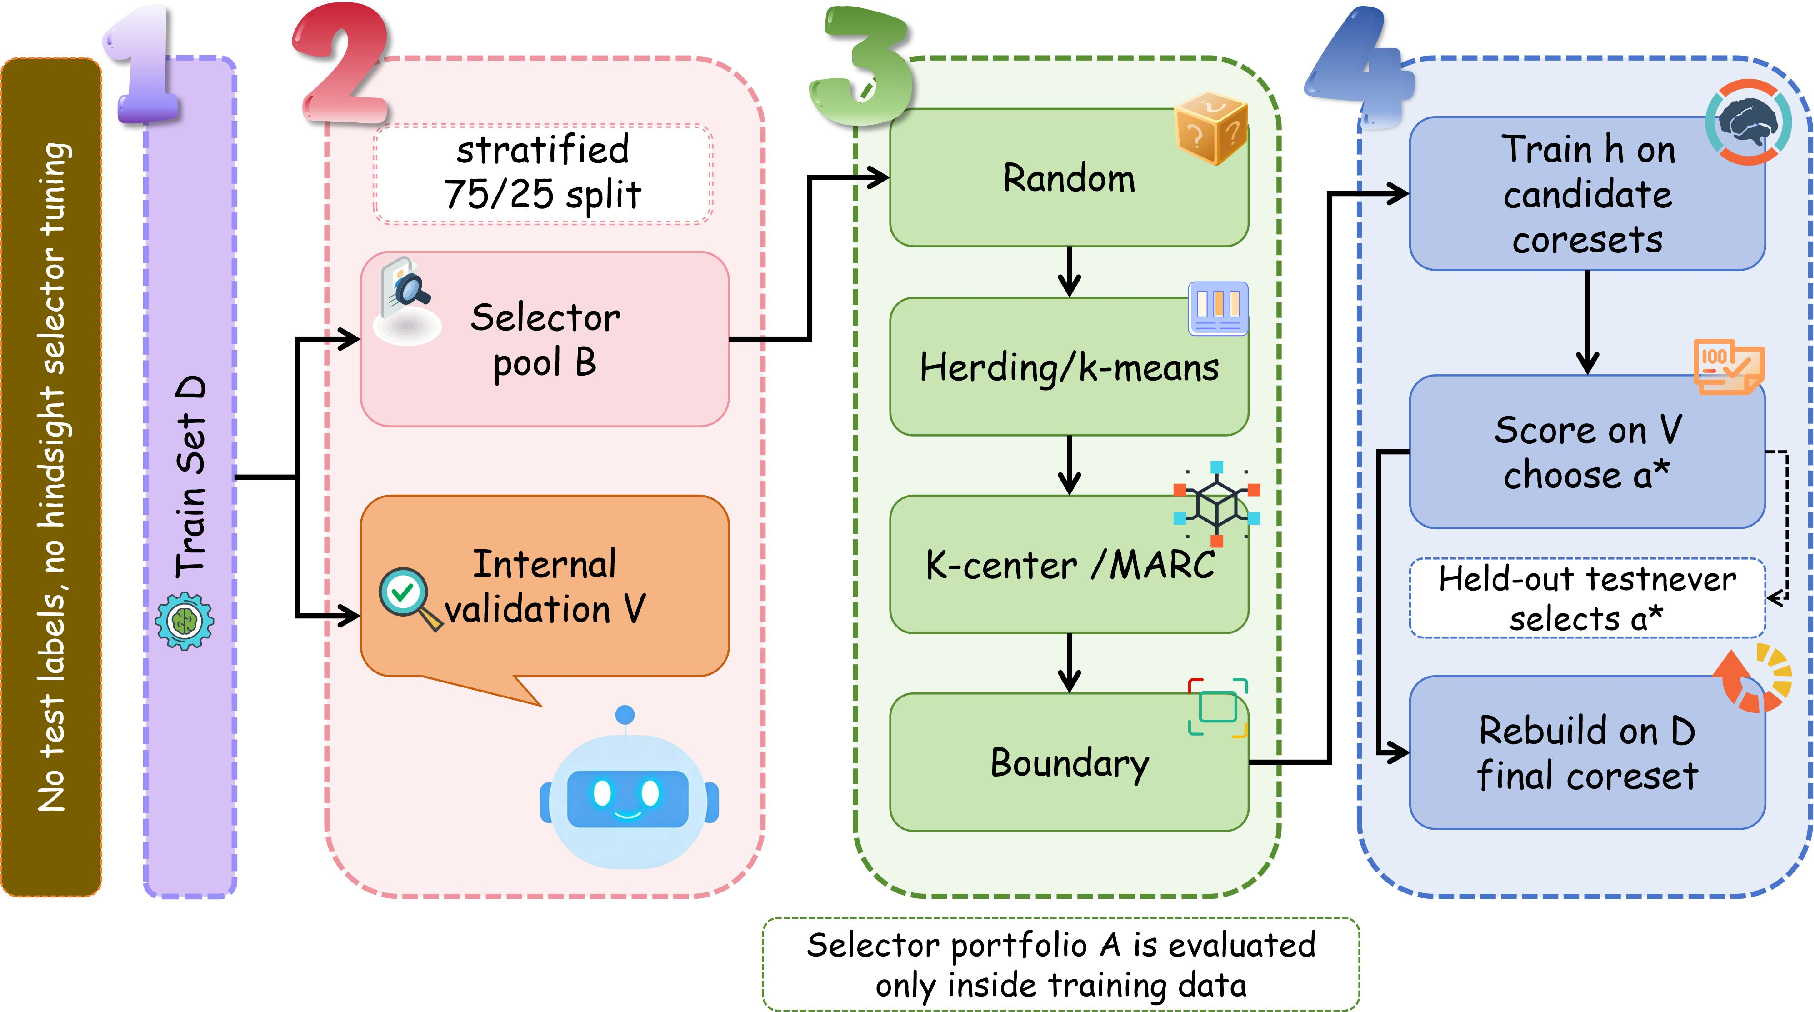
\includegraphics[width=0.98\linewidth]{../figures/Figure_1_vacs_workflow.pdf}
\caption{\textbf{Training-only VACS workflow.} Candidate selectors are evaluated on internal validation splits drawn from the training data. The held-out test set is used only for final evaluation. After the selector has been chosen, the selected rule is rebuilt on the full outer training split.}
\label{fig:workflow}
\end{figure}

VACS-R repeats the internal validation-ranking step five times with independently stratified 75/25 pool-validation splits, averages each selector's validation accuracy and macro-F1, and then applies the selected rule once to the full training split. VACS-F is the low-cost diagnostic protocol. VACS-R is the stability-oriented protocol when extra selector-choice time is acceptable.

\subsection*{Low-budget benchmark performance}

The main benchmark uses five public datasets available through scikit-learn: digits, iris, wine, breast cancer, and the full 20-class 20 Newsgroups corpus. The main analysis averages budgets of one and two examples per class across eight random seeds and five datasets, producing 80 matched low-budget units. A distance-weighted 3-nearest-neighbour classifier is trained on the selected examples.

The fast protocol reaches 70.6\% mean accuracy, numerically tying the best pooled static selector, herding (Table~\ref{tab:low_budget}). The unrounded paired difference is only +0.02 percentage points. A bootstrap interval over the matched low-budget units is [-1.38,+1.20] points, so VACS-F should be read as a near-tie rather than a mean-effect win. Boundary-only selection reaches 32.2\%, and the BADGE-inspired uncertainty-diversity comparator reaches 38.9\%, showing that boundary or uncertainty-diversity bias alone is not sufficient under this tiny selected-label budget.

\begin{table}[H]
\centering
\caption{\textbf{Low-budget performance over budgets one and two.} Values are percentages averaged over five datasets and eight random seeds. VACS here denotes the fast single-split protocol, VACS-F.}
\label{tab:low_budget}
\small
\begin{tabular}{lcccc}
\toprule
Method & Acc. & Std. & Macro-F1 & F1 Std. \\
\midrule
VACS & \textbf{70.6} & \textbf{31.7} & \textbf{70.2} & \textbf{32.1} \\
Herding & 70.6 & 33.4 & 69.5 & 35.2 \\
MARC & 70.6 & 33.4 & 69.4 & 35.1 \\
K-means & 70.3 & 33.3 & 69.1 & 35.0 \\
K-center & 67.3 & 32.1 & 65.8 & 33.8 \\
Random & 65.9 & 29.1 & 64.8 & 29.8 \\
BADGE & 38.9 & 23.1 & 37.5 & 22.7 \\
Boundary & 32.2 & 21.5 & 31.3 & 21.0 \\
\bottomrule
\end{tabular}

\end{table}

The selector choices are heterogeneous (Figure~\ref{fig:selector_mix}). On full 20-class 20 Newsgroups, VACS-F chooses boundary selection in 9 of 16 low-budget units and random selection in the other 7. Dense datasets more often route to representative rules such as herding, k-means, and MARC. This supports the premise that the best selector bias is not fixed across data regimes, while also identifying a sparse-text failure boundary: in a compact full-20-class TF-IDF stress summary, VACS reaches 9.7\% and static random reaches 12.1\%.

\begin{figure}[H]
\centering
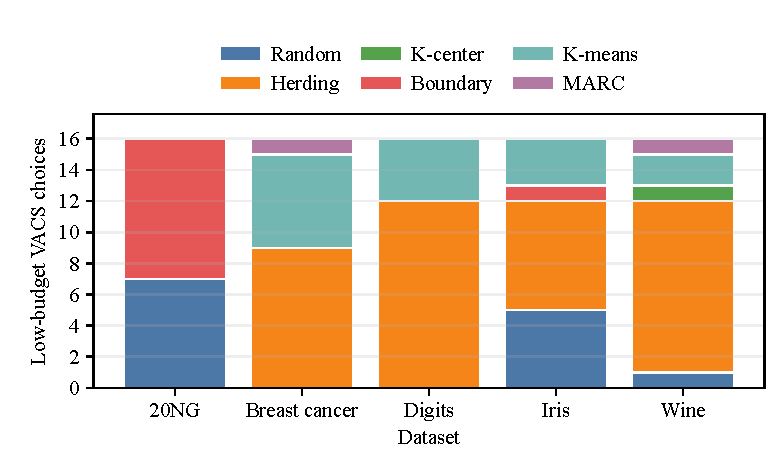
\includegraphics[width=0.98\linewidth]{../figures/Figure_2_selector_mix.pdf}
\caption{\textbf{Selector choices in the low-budget regime.} VACS-F uses different selector biases across datasets. The pattern is mechanism evidence rather than proof of universal dominance.}
\label{fig:selector_mix}
\end{figure}

\subsection*{Repeated validation improves the deployable protocol}

The strongest positive evidence comes from VACS-R. On the same 80 matched low-budget units, VACS-R reaches 72.1\% pooled accuracy and improves over herding by +1.54 points, with a 95\% bootstrap interval of [+0.68,+2.49] and a 30/43/7 win/tie/loss pattern. Against a stricter non-deployable reference that chooses the best static selector separately for each dataset using hindsight, VACS-R is essentially tied at -0.13 points with interval [-0.42,+0.15] (Table~\ref{tab:repeated}). Thus VACS-R is the strongest evaluated training-only deployable protocol in this study, but it does not exceed a hindsight-tuned static rule.

\begin{table}[H]
\centering
\caption{\textbf{Paired audit for the repeated-validation protocol.} The per-dataset static reference is a non-deployable hindsight diagnostic, not a usable baseline for deployment. Values are percentages except for the paired delta and confidence interval, which are percentage points.}
\label{tab:repeated}
\small
\begin{tabular}{lccccc}
\toprule
Reference & $n$ & Repeated VACS & Ref. & $\Delta$ [95\% CI] & W/T/L \\
\midrule
Herding & 80 & \textbf{72.1} & 70.6 & +1.54 [+0.68,+2.49] & 30/43/7 \\
Per-dataset static & 80 & \textbf{72.1} & 72.3 & -0.13 [-0.42,+0.15] & 5/67/8 \\
\bottomrule
\end{tabular}

\end{table}

Validation-size diagnostics confirm that the result depends on the internal validation protocol but is not driven by one unchecked split. A reliability diagnostic at 10\%, 20\%, 25\%, and 33\% validation fractions reports pooled gains over herding of +0.94, +0.10, +1.13, and +0.86 points, respectively. A separate split-sensitivity rerun at 20\%, 25\%, and 33\% reports gains of -0.90, +0.02, and +0.56 points. The 20\% split is the weakest and nearly tied, while the repeated protocol reduces split-ranking noise. Figure~\ref{fig:protocol} summarizes the validation-fraction and repeat-validation evidence.

\begin{figure}[H]
\centering
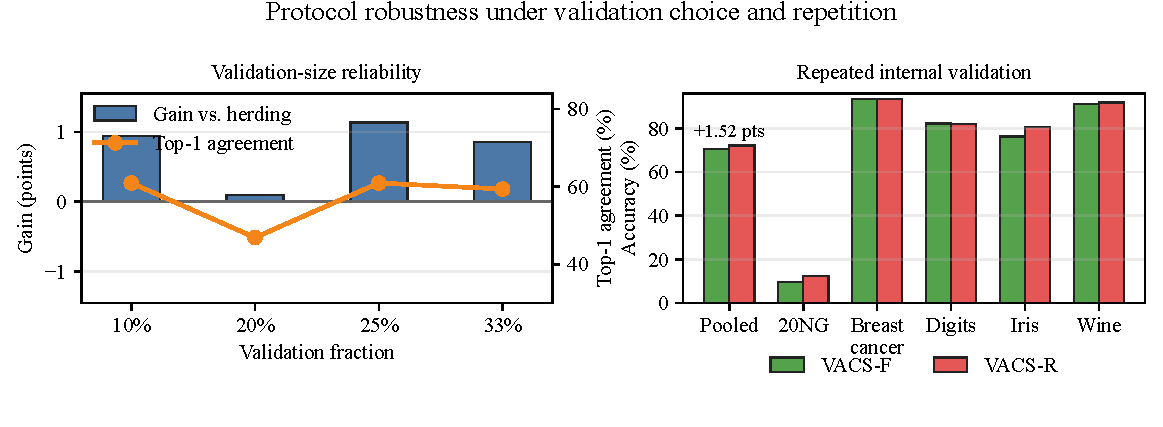
\includegraphics[width=0.98\linewidth]{../figures/Figure_3_protocol_robustness.pdf}
\caption{\textbf{Protocol robustness.} Left: validation-size sensitivity and selector agreement. Right: pooled and dataset-level VACS-F versus VACS-R accuracy.}
\label{fig:protocol}
\end{figure}

\subsection*{External Covertype audit}

A larger tabular audit uses the UCI Covertype dataset \citep{blackard1998covertype}. The confirmatory rerun samples 62,240 examples, covers all seven classes, uses 16 random seeds and budgets one and two, and produces 32 matched seed-budget units. VACS-R reaches 44.0\% mean accuracy, improves over herding by +5.42 points with a 95\% bootstrap interval of [+3.52,+7.33], and has a 16/16/0 win/tie/loss pattern against herding. However, VACS-R exactly matches MARC at +0.00 points with a 0/32/0 pattern (Table~\ref{tab:covtype}). The audit therefore supports avoidance of a weak static default, not superiority over the best static bias in the portfolio.

\begin{table}[H]
\centering
\caption{\textbf{Confirmatory Covertype audit.} The audit uses a fresh 62,240-example stratified sample and 32 matched seed-budget units. Values are percentages except for paired notes.}
\label{tab:covtype}
\small
\begin{tabular}{lcccc}
\toprule
Method & Acc. & Macro-F1 & Selected & Paired note \\
\midrule
Random & 33.8 & 32.6 & 10.5 &  \\
Herding & 38.6 & 37.1 & 10.5 &  \\
K-center & 38.0 & 37.1 & 10.5 &  \\
Boundary & 20.5 & 17.2 & 10.5 &  \\
K-means & 42.8 & 41.7 & 10.5 &  \\
MARC & 44.0 & 42.8 & 10.5 &  \\
VACS-F & \textbf{44.0} & \textbf{42.7} & \textbf{10.5} & vs. Herding +5.35 [+3.48,+7.23] \\
VACS-R & \textbf{44.0} & \textbf{42.8} & \textbf{10.5} & vs. Herding +5.42 [+3.52,+7.33] \\
\bottomrule
\end{tabular}

\end{table}

\subsection*{Boundary evidence and cost}

Several checks define the limit of the claim. VACS-F trails a per-dataset hindsight static selector by -1.64 points over 80 low-budget units, with a 95\% bootstrap interval of [-2.98,-0.61]. VACS-R removes most of that gap but does not beat the hindsight reference. Frozen text-embedding probes on full 20-class 20 Newsgroups are boundary evidence rather than positive modern-embedding support: a Qwen2.5-0.5B-Instruct probe reports 40.13\% for VACS versus 40.24\% for herding, a DeBERTa probe reports 9.76\% versus 9.93\% for herding, and SmolLM2 probes are near ties or slight losses. Frozen image-embedding probes also tie herding: Fashion-MNIST with ConvNeXt-Tiny reaches 75.60\% for both VACS and herding, and CIFAR-10 with ResNet18 reaches 64.73\% for both.

The wrapper has measurable selection cost. Across the 80 low-budget decisions in the main run, herding selection takes 10.47 seconds, whereas VACS-F spends 79.82 seconds on validation and 7.39 seconds on the final rebuild, for 87.21 seconds total. The main CPU run records 1910.75 seconds. VACS-R intentionally spends more selector-choice time by repeating internal validation.

\section*{Discussion}

The main finding is that selector choice is a real source of variance in extreme few-shot classification. A single fixed selector can be strong on average, but its bias may be mismatched to a particular representation or budget. VACS uses training-only validation to select among several simple biases. The fast version is essentially tied with the best pooled static rule, while the repeated version gives the clearest positive deployable result in this study.

The evidence is intentionally bounded. VACS-R improves over herding in the pooled low-budget protocol, but it only ties a non-deployable hindsight static reference and exactly ties MARC on Covertype. Frozen transformer and image-embedding probes do not establish a broad modern-representation advantage. These results argue against a universal coreset claim and for a narrower scientific claim: under extremely small class-balanced budgets, repeated internal validation can choose between selector biases competitively without using test labels.

This has practical implications for small-data pipelines. When a practitioner must retain one or two examples per class, reporting only one static selector can hide substantial selector mismatch. A finite validation portfolio provides a transparent diagnostic, and the validation gap can be used as an audit signal when candidate selectors are nearly tied. The cost is also visible: VACS-R is most appropriate when additional selector-choice time is acceptable and reliability matters.

Future work should test predeclared selector-decision rules on larger modern benchmarks, retrieval and prompt-selection tasks, and deep representation settings where the current boundary probes mostly tie static selectors. The saved-score meta-selector sweep in the project package identifies one such direction, but it is deliberately not used as a main result because it was found post hoc.

\section*{Methods}

\subsection*{Problem definition}

Let a labelled training set be $\D=\{(x_i,y_i)\}_{i=1}^n$, where $x_i \in \mathbb{R}^d$ and $y_i$ belongs to a finite class set. A selector receives $\D$ and a per-class budget $b$, and returns a subset $\Sset$ with at most $b$ examples per class. A downstream classifier is trained only on selected examples. The goal is high held-out performance for the downstream classifier under the small selected-label budget.

\subsection*{Selector portfolio}

The VACS portfolio contains random selection, herding, k-center, boundary selection, k-means medoids, and MARC. Random selection samples uniformly without replacement within each class. Herding selects the examples closest to the class centroid. K-center uses farthest-first traversal within each class, initialized near the class centroid. K-means medoids fit deterministic class-conditional k-means and map centers back to real examples. Boundary selection computes a centroid-margin score and selects the lowest-margin examples. The BADGE-inspired external comparator uses gradient embeddings from a regularized linear logistic-regression surrogate \citep{ash2020deep}; it is not part of the final VACS portfolio.

MARC, the margin-weighted representative selector, fits the same deterministic medoid routine as k-means but weights each within-class example by a transformed centroid margin. For an example $x_i$ in class $y_i$, the centroid margin is
\begin{equation}
m_i=\min_{y \neq y_i}\|x_i-c_y\|_2^2-\|x_i-c_{y_i}\|_2^2,
\end{equation}
where $c_y$ is the centroid of class $y$. Margins are standardized within the class and converted to positive weights
\begin{equation}
w_i=0.2+\frac{1.8}{1+\exp(-z_i)}, \qquad
z_i=\frac{m_i-\operatorname{median}(m)}{\operatorname{std}(m)+10^{-8}}.
\end{equation}
Thus ambiguous examples have less influence on representative centers, rather than being directly selected as boundary points.

\subsection*{VACS-F and VACS-R}

For VACS-F, each outer training split is stratified into a selector pool $\Bset$ and an internal validation set $\Vset$ using a 75/25 split. For each selector $a \in \Aset$, the selector constructs a class-balanced subset from $\Bset$, the downstream classifier is trained on that subset, and accuracy and macro-F1 are evaluated on $\Vset$. The winning selector is chosen by validation accuracy, then macro-F1, then a fixed selector order. The selected rule is then rerun on the full outer training split $\D$ to produce the final coreset.

For VACS-R, this validation-scoring step is repeated five times with independently stratified 75/25 internal splits. Each selector's validation accuracy and macro-F1 are averaged across repeats before selecting the final rule. The final coreset is again rebuilt once from the full outer training split.

\subsection*{Datasets and preprocessing}

The main benchmark uses scikit-learn \citep{pedregosa2011scikit}: digits, iris, wine, breast cancer, and the full 20-class 20 Newsgroups corpus. Dense features are standardized and L2-normalized after each outer train/test split. For 20 Newsgroups, raw documents are split first; TF-IDF is then fit only on the outer training documents, capped at 3,000 dimensions, and applied to held-out test documents. Each dataset uses stratified 70/30 train/test splits and seeds 0 through 7.

The Covertype audit uses the UCI forest cover type dataset \citep{blackard1998covertype}. The first audit samples 32,747 examples capped at 5,000 per class. The confirmatory audit samples 62,240 examples with a larger cap, a fresh sample seed, 16 random seeds, and budgets one and two. Both audits use the same selector portfolio, preprocessing discipline, 70/30 outer splits, VACS-F, VACS-R, and distance-weighted 3-nearest-neighbour evaluation.

\subsection*{Evaluation and statistics}

The main downstream model is a distance-weighted 3-nearest-neighbour classifier. If fewer than three total examples are selected, the neighbour count is reduced accordingly. The main outcome is accuracy; macro-F1 is reported as a secondary metric. The primary comparison focuses on budgets one and two examples per class. Paired differences are computed over matched dataset-seed-budget units. Bootstrap confidence intervals use resampling over matched units, and win/tie/loss counts report the sign of each paired difference.

\subsection*{Software and reproducibility}

The experiments are implemented in Python with scikit-learn and standard scientific Python libraries. The package includes scripts that regenerate the main experiment, validation-size diagnostics, the repeated-validation audit, the Covertype audits, the figure files, and claim-consistency checks. The figures in this manuscript are generated with Times New Roman embedded in the PDF figure text, including axis labels.

\subsection*{AI-assisted preparation}

An AI assistant was used to help draft and reorganize the manuscript, prepare submission checklists, and audit consistency between the text and generated result files. Human authors remain responsible for verifying the manuscript, code, data, references, and all conclusions before submission.

\section*{Data availability}

All primary datasets used in this study are public. Digits, iris, wine, breast cancer, and 20 Newsgroups are accessed through scikit-learn. Covertype is available from the UCI Machine Learning Repository. The generated result tables, manifests, and figure files used in this manuscript are included with the submission package and can be regenerated from the provided scripts.

\section*{Code availability}

The code required to reproduce the experiments, tables, figures, and consistency checks is included in the project package and is available from the public GitHub repository below.

\url{https://github.com/HaotongLuan/validation-aligned-coreset-selection}

The main driver is \texttt{experiments/run\_vacs\_experiments.py}; companion scripts rerun the Covertype audits, repeated-validation diagnostics, validation-size diagnostics, and figure generation. An archive DOI will be added if one is created for the public release.

\section*{Acknowledgements}

This work was supported by the National College Students’ Innovation and Entrepreneurship Training Program of Shenzhen Technology University (2026).

\section*{Author contributions}

[Author-specific contributions to be completed by the authors before submission.]

\section*{Competing interests}

[Competing-interest statement to be confirmed by all authors before submission.]

\section*{Additional information}

Correspondence and requests for materials should be addressed to the corresponding author listed on the title page.

\begin{thebibliography}{31}
\providecommand{\natexlab}[1]{#1}
\providecommand{\url}[1]{\texttt{#1}}
\expandafter\ifx\csname urlstyle\endcsname\relax
  \providecommand{\doi}[1]{doi: #1}\else
  \providecommand{\doi}{doi: \begingroup \urlstyle{rm}\Url}\fi

\bibitem[Lewis and Gale(1994)]{lewis1994sequential}
David~D. Lewis and William~A. Gale.
\newblock A sequential algorithm for training text classifiers.
\newblock In \emph{Proceedings of the 17th Annual International ACM SIGIR
  Conference on Research and Development in Information Retrieval}, pages 3--12,
  1994.

\bibitem[Freund et~al.(1997)Freund, Seung, Shamir, and Tishby]{freund1997query}
Yoav Freund, H.~Sebastian Seung, Eli Shamir, and Naftali Tishby.
\newblock Selective sampling using the query by committee algorithm.
\newblock \emph{Machine Learning}, 28:\penalty0 133--168, 1997.

\bibitem[Settles(2009)]{settles2009active}
Burr Settles.
\newblock Active learning literature survey.
\newblock \emph{Computer Sciences Technical Report 1648, University of
  Wisconsin--Madison}, 2009.

\bibitem[Sener and Savarese(2018)]{sener2018active}
Ozan Sener and Silvio Savarese.
\newblock Active learning for convolutional neural networks: A core-set
  approach.
\newblock In \emph{International Conference on Learning Representations}, 2018.

\bibitem[Ash et~al.(2020)Ash, Zhang, Krishnamurthy, Langford, and
  Agarwal]{ash2020deep}
Jordan~T. Ash, Chicheng Zhang, Akshay Krishnamurthy, John Langford, and Alekh
  Agarwal.
\newblock Deep batch active learning by diverse, uncertain gradient lower
  bounds.
\newblock In \emph{International Conference on Learning Representations}, 2020.

\bibitem[Feldman(2020)]{feldman2020coresets}
Dan Feldman.
\newblock Core-sets: An updated survey.
\newblock \emph{Wiley Interdisciplinary Reviews: Data Mining and Knowledge
  Discovery}, 10\penalty0 (1):\penalty0 e1335, 2020.

\bibitem[Wei et~al.(2015)Wei, Iyer, and Bilmes]{wei2015submodularity}
Kai Wei, Rishabh Iyer, and Jeff Bilmes.
\newblock Submodularity in data subset selection and active learning.
\newblock In \emph{Proceedings of the 32nd International Conference on Machine
  Learning}, volume~37 of \emph{Proceedings of Machine Learning Research}, pages
  1954--1963, 2015.

\bibitem[Bachem et~al.(2017)Bachem, Lucic, and Krause]{bachem2017practical}
Olivier Bachem, Mario Lucic, and Andreas Krause.
\newblock Practical coreset constructions for machine learning.
\newblock arXiv:1703.06476, 2017.

\bibitem[Mirzasoleiman et~al.(2020)Mirzasoleiman, Bilmes, and
  Leskovec]{mirzasoleiman2020craig}
Baharan Mirzasoleiman, Jeff~A. Bilmes, and Jure Leskovec.
\newblock Coresets for data-efficient training of machine learning models.
\newblock In \emph{Proceedings of the 37th International Conference on Machine
  Learning}, volume 119 of \emph{Proceedings of Machine Learning Research},
  pages 6950--6960, 2020.

\bibitem[Killamsetty et~al.(2021{\natexlab{a}})Killamsetty, Sivasubramanian,
  Ramakrishnan, and Iyer]{killamsetty2021glister}
Krishnateja Killamsetty, Durga Sivasubramanian, Ganesh Ramakrishnan, and
  Rishabh Iyer.
\newblock GLISTER: Generalization based data subset selection for efficient and
  robust learning.
\newblock In \emph{Proceedings of the AAAI Conference on Artificial
  Intelligence}, volume~35, pages 8110--8118, 2021{\natexlab{a}}.

\bibitem[Killamsetty et~al.(2021{\natexlab{b}})Killamsetty, Durga,
  Ramakrishnan, De, and Iyer]{killamsetty2021gradmatch}
Krishnateja Killamsetty, S.~Durga, Ganesh Ramakrishnan, Abir De, and Rishabh
  Iyer.
\newblock GradMatch: Gradient matching based data subset selection for efficient
  deep model training.
\newblock In \emph{Proceedings of the 38th International Conference on Machine
  Learning}, volume 139 of \emph{Proceedings of Machine Learning Research},
  pages 5464--5474, 2021{\natexlab{b}}.

\bibitem[Cover and Hart(1967)]{cover1967nearest}
Thomas Cover and Peter Hart.
\newblock Nearest neighbor pattern classification.
\newblock \emph{IEEE Transactions on Information Theory}, 13\penalty0
  (1):\penalty0 21--27, 1967.

\bibitem[Hart(1968)]{hart1968condensed}
P.~E. Hart.
\newblock The condensed nearest neighbor rule.
\newblock \emph{IEEE Transactions on Information Theory}, 14\penalty0
  (3):\penalty0 515--516, 1968.

\bibitem[Wilson(1972)]{wilson1972edited}
D.~L. Wilson.
\newblock Asymptotic properties of nearest neighbor rules using edited data.
\newblock \emph{IEEE Transactions on Systems, Man, and Cybernetics},
  2\penalty0 (3):\penalty0 408--421, 1972.

\bibitem[Brighton and Mellish(2002)]{brighton2002advances}
Henry Brighton and Chris Mellish.
\newblock Advances in instance selection for instance-based learning algorithms.
\newblock \emph{Data Mining and Knowledge Discovery}, 6:\penalty0 153--172,
  2002.

\bibitem[Olvera-L{\'o}pez et~al.(2010)Olvera-L{\'o}pez, Carrasco-Ochoa,
  Mart{\'i}nez-Trinidad, and Kittler]{olvera2010review}
J.~Arturo Olvera-L{\'o}pez, J.~Ariel Carrasco-Ochoa, J.~Francisco
  Mart{\'i}nez-Trinidad, and Josef Kittler.
\newblock A review of instance selection methods.
\newblock \emph{Artificial Intelligence Review}, 34:\penalty0 133--143, 2010.

\bibitem[Garc{\'i}a et~al.(2012)Garc{\'i}a, Derrac, Cano, and
  Herrera]{garcia2012prototype}
Salvador Garc{\'i}a, Joaqu{\'i}n Derrac, Jos{\'e}~Ram{\'o}n Cano, and
  Francisco Herrera.
\newblock Prototype selection for nearest neighbor classification: Taxonomy and
  empirical study.
\newblock \emph{IEEE Transactions on Pattern Analysis and Machine Intelligence},
  34\penalty0 (3):\penalty0 417--435, 2012.

\bibitem[Vinyals et~al.(2016)Vinyals, Blundell, Lillicrap, Wierstra, and
  others]{vinyals2016matching}
Oriol Vinyals, Charles Blundell, Timothy Lillicrap, Daan Wierstra, and others.
\newblock Matching networks for one shot learning.
\newblock In \emph{Advances in Neural Information Processing Systems}, volume~29,
  2016.

\bibitem[Finn et~al.(2017)Finn, Abbeel, and Levine]{finn2017maml}
Chelsea Finn, Pieter Abbeel, and Sergey Levine.
\newblock Model-agnostic meta-learning for fast adaptation of deep networks.
\newblock In \emph{Proceedings of the 34th International Conference on Machine
  Learning}, volume~70 of \emph{Proceedings of Machine Learning Research}, pages
  1126--1135, 2017.

\bibitem[Snell et~al.(2017)Snell, Swersky, and Zemel]{snell2017prototypical}
Jake Snell, Kevin Swersky, and Richard~S. Zemel.
\newblock Prototypical networks for few-shot learning.
\newblock In \emph{Advances in Neural Information Processing Systems}, 2017.

\bibitem[Sung et~al.(2018)Sung, Yang, Zhang, Xiang, Torr, and
  Hospedales]{sung2018relation}
Flood Sung, Yongxin Yang, Li~Zhang, Tao Xiang, Philip H.~S. Torr, and
  Timothy~M. Hospedales.
\newblock Learning to compare: Relation network for few-shot learning.
\newblock In \emph{Proceedings of the IEEE Conference on Computer Vision and
  Pattern Recognition}, pages 1199--1208, 2018.

\bibitem[Stone(1974)]{stone1974cross}
M.~Stone.
\newblock Cross-validatory choice and assessment of statistical predictions.
\newblock \emph{Journal of the Royal Statistical Society: Series B},
  36\penalty0 (2):\penalty0 111--133, 1974.

\bibitem[Kohavi(1995)]{kohavi1995study}
Ron Kohavi.
\newblock A study of cross-validation and bootstrap for accuracy estimation and
  model selection.
\newblock In \emph{Proceedings of the Fourteenth International Joint Conference
  on Artificial Intelligence}, pages 1137--1143, 1995.

\bibitem[Dietterich(1998)]{dietterich1998statistical}
Thomas~G. Dietterich.
\newblock Approximate statistical tests for comparing supervised classification
  learning algorithms.
\newblock \emph{Neural Computation}, 10\penalty0 (7):\penalty0 1895--1923,
  1998.

\bibitem[Nadeau and Bengio(2003)]{nadeau2003inference}
Claude Nadeau and Yoshua Bengio.
\newblock Inference for the generalization error.
\newblock \emph{Machine Learning}, 52:\penalty0 239--281, 2003.

\bibitem[Dror et~al.(2018)Dror, Baumer, Bogomolov, and Reichart]{dror2018hitchhiker}
Rotem Dror, Gili Baumer, Segev Bogomolov, and Roi Reichart.
\newblock The hitchhiker's guide to testing statistical significance in natural
  language processing.
\newblock In \emph{Proceedings of the 56th Annual Meeting of the Association
  for Computational Linguistics}, pages 1383--1392, 2018.

\bibitem[Rice(1976)]{rice1976algorithm}
John~R. Rice.
\newblock The algorithm selection problem.
\newblock \emph{Advances in Computers}, 15:\penalty0 65--118, 1976.

\bibitem[Kotthoff(2014)]{kotthoff2014algorithm}
Lars Kotthoff.
\newblock Algorithm selection for combinatorial search problems: A survey.
\newblock \emph{AI Magazine}, 35\penalty0 (3):\penalty0 48--60, 2014.

\bibitem[Thornton et~al.(2013)Thornton, Hutter, Hoos, and
  Leyton-Brown]{thornton2013autoweka}
Chris Thornton, Frank Hutter, Holger~H. Hoos, and Kevin Leyton-Brown.
\newblock Auto-WEKA: Combined selection and hyperparameter optimization of
  classification algorithms.
\newblock In \emph{Proceedings of the 19th ACM SIGKDD International Conference
  on Knowledge Discovery and Data Mining}, pages 847--855, 2013.

\bibitem[Blackard and Dean(1998)]{blackard1998covertype}
Jock~A. Blackard and Denis~J. Dean.
\newblock Covertype.
\newblock UCI Machine Learning Repository, 1998.

\bibitem[Pedregosa et~al.(2011)Pedregosa, Varoquaux, Gramfort, Michel, Thirion,
  Grisel, Blondel, Prettenhofer, Weiss, Dubourg, Vanderplas, Passos,
  Cournapeau, Brucher, Perrot, and Duchesnay]{pedregosa2011scikit}
Fabian Pedregosa, Ga{\"e}l Varoquaux, Alexandre Gramfort, Vincent Michel,
  Bertrand Thirion, Olivier Grisel, Mathieu Blondel, Peter Prettenhofer, Ron
  Weiss, Vincent Dubourg, Jake Vanderplas, Alexandre Passos, David Cournapeau,
  Matthieu Brucher, Matthieu Perrot, and {\'E}douard Duchesnay.
\newblock Scikit-learn: Machine learning in python.
\newblock \emph{Journal of Machine Learning Research}, 12:\penalty0 2825--2830,
  2011.

\end{thebibliography}

\end{document}
